%!TEX root = ../template.tex
%%%%%%%%%%%%%%%%%%%%%%%%%%%%%%%%%%%%%%%%%%%%%%%%%%%%%%%%%%%%%%%%%%%%
%% chapter3.tex
%% NOVA thesis document file
%%
%% Chapter with a short latex tutorial and examples
%%%%%%%%%%%%%%%%%%%%%%%%%%%%%%%%%%%%%%%%%%%%%%%%%%%%%%%%%%%%%%%%%%%%

\typeout{NT FILE chapter3.tex}%

\chapter{State Of The Art}
\label{cha:State_Of_The_Art}

The State-Of-The-Art outlines the most relevant and advanced work currently available in the area covered by this work. 
It provides an overview of existing research, tools, and methodologies, helping to frame the context in which this work is situated. 
By reviewing what has already been accomplished, this section highlights ongoing challenges and uncovers the gaps that this work 
aims to address.

\section{Certified Compilers}
\label{sec:Certified_Compilers}

A compiler is a software system that translates a program written in a source programming language into an equivalent representation 
in a target language, typically a lower-level language such as assembly or machine code. The goal of a compiler is not only to preserve 
the semantics of the original program but also to generate efficient and executable code for the target platform.~\cite{AhoSU86}

A central challenge in compiler technology is: How can we trust compilers?. As discussed previously, compilers are 
inherently complex systems, particularly optimizing compilers, which perform intricate symbolic transformations. 
Despite rigorous testing practices, compilers can still introduce subtle bugs during these transformations. Such bugs are often 
extremely difficult to detect and diagnose~\cite{Leroy09-back-end}, as they may lead to unexpected program crashes, 
incorrect behaviour, or silent miscomputations in the generated code, even when the original source code remains syntactically and 
semantically valid.

This raises serious concerns in the context of safety-critical or high-assurance software, where traditional validation 
through testing alone is insufficient. In such domains, testing must be complemented or in some cases replaced by formal methods, 
such as model checking, static analysis, and deductive program verification~\cite{Leroy09-back-end}.

This is precisely where certified compilers become essential. A certified compiler is accompanied by a machine-checked formal proof 
that guarantees semantic preservation during the transformation from source to target code. It preserves the semantics of the source 
program during its transformation into target code. This approach offers strong assurances about the absence of certain classes of 
errors, such as compilation bugs, compilation inaccuracies, or unsafe optimizations~\cite{Leroy09}. Unlike traditional compilers, 
whose correctness is typically established through empirical testing or informal reasoning, certified compilers provide mathematical 
guarantees of correctness, making them valuable in the development of high-assurance and safety-critical software.

\subsection{CompCert}
\label{sec:CompCert}

The development of a realistic and verified compiler began with \compcert. Here, verified denotes a compiler accompanied by
a machine-checked proof that the generated code behaves exactly as prescribed by the semantics of the source program.
Realistic refers to a compiler that can be effectively employed in the production of critical software systems~\cite{Leroy09-back-end}.

\compcert adopts a multi-pass compilation architecture, where each pass translates an intermediate representation into a lower-level 
form, gradually transforming the high-level C source code into target assembly code. These intermediate languages are Clight, Cminor, 
RTL, LTL, and others which are formally defined within Coq~\cite{75277.75285}. \compcert's core is implemented in Gallina, the 
functional programming language of Coq, which is based on the Calculus of Inductive Constructions, a powerful higher-order logic and 
typed $\lambda$-calculus. 
This implementation enables formal reasoning and machine-checked proofs of correctness for each compilation phase~\cite{MonniauxB22}.

Although \compcert is developed in Coq, it is not executed within the proof assistant. Instead, the verified Gallina code is extracted 
to \ocaml, where it is combined with a small portion of handwritten \ocaml code to produce an efficient and executable 
compiler~\cite{MonniauxB22}.

Since the compiler must generate a large subset of the C language, the code needs to be efficient enough and compact enough to fit the 
requirements of critical embedded systems. This implies a multi-pass compiler that features good register allocation and some basic 
optimizations~\cite{Leroy09-back-end}. The pipeline for the compiler is presented below:

\begin{figure}[H]
    \centering
    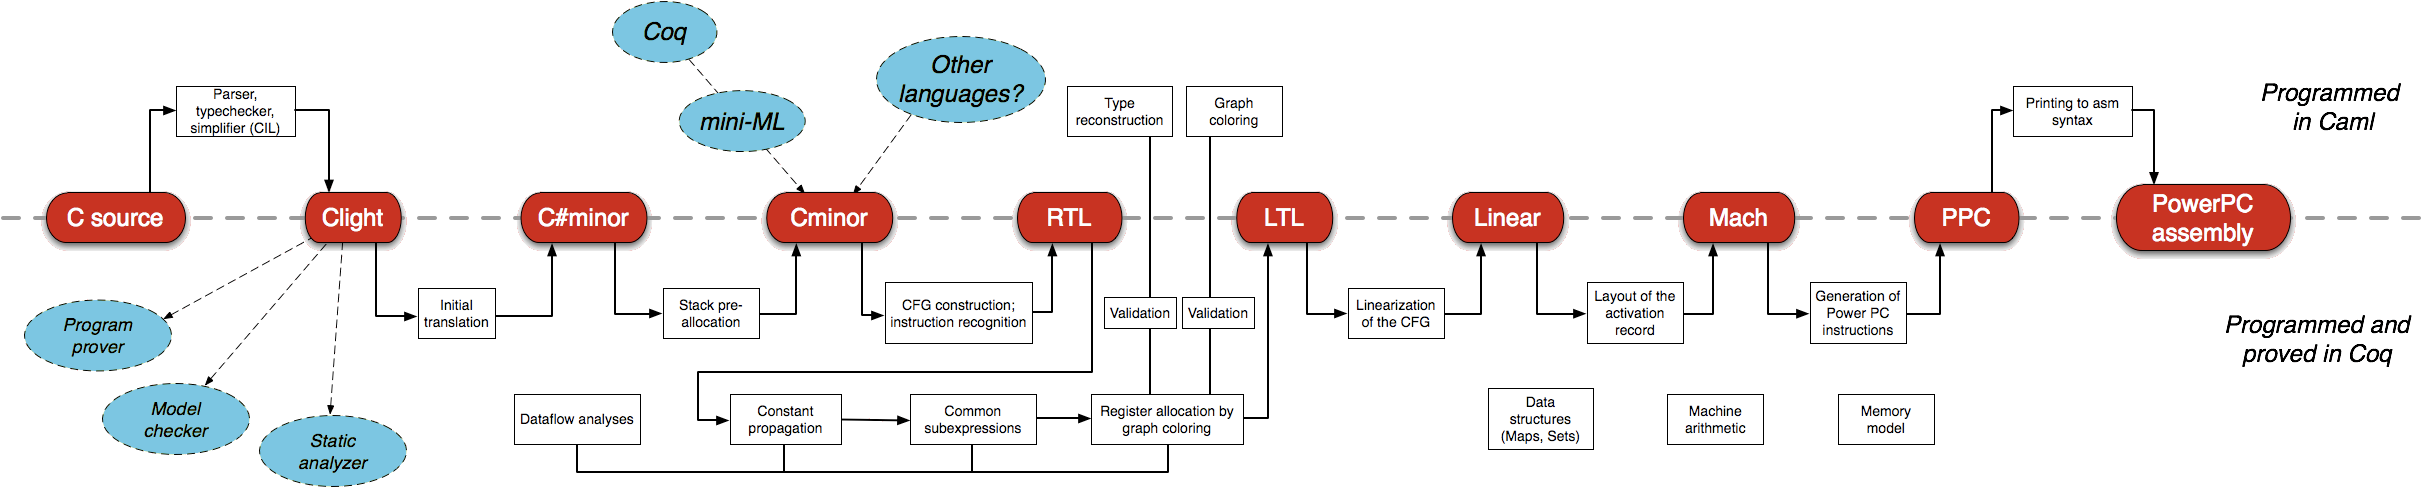
\includegraphics[width=\linewidth]{images/compcert_diagram.png}
    \caption{\compcert pipeline diagram~\cite{hal-01643290, CompCertPipeline}}
    \label{fig:CompCertPipeline}
\end{figure}

\subsection{CakeML}
\label{sec:CakeML}

The \cml compiler stands out as one of the most realistic verified compilers for functional programming. Inspired by both CompCert 
and \ocaml compilers, it supports a rich set of language features commonly found in unverified compilers for functional languages. The 
main goal of the \cml compiler is to combine end-to-end formal verification with practical performance, making it suitable 
for high-assurance applications without compromising efficiency~\cite{TanMKFON19}. \cml is a formally verified functional programming 
language and compiler tool chain, specifically designed to target practical, off-the-shelf hardware while achieving a high degree of 
trustworthiness. It serves as a robust platform for software in domains where correctness is paramount. By focusing on functional 
programming and end-to-end verification, \cml complements \compcert, which primarily target imperative languages and emphasize 
performance oriented optimizations. Together, these approaches address different but complementary aspects of verified software 
development~\cite{POPL14}.

The programming language used in \cml is a subset of Standard ML, which is
a functional programming language that fully embraces the expressiveness of mathematical functions. 
However, it was also shaped by practical programming needs, leading to the inclusion of imperative constructs and a 
robust exception handling system. The language supports modularity through an advanced system of parametric modules, 
designed to facilitate the structured development of large-scale software systems. Moreover, Standard ML is strongly 
and statically typed, and it was the first programming language to introduce a form of polymorphic type inference that 
combines strong type safety with considerable flexibility in programming style ~\cite{milner1997definition}.

One of the most distinguishing features of Standard ML is its formal definition, which precisely specifies the language's 
static and dynamic semantics using structural operational semantics~\cite{milner1997definition}, which played a key role in laying the 
groundwork for end-to-end verified compilers~\cite{Syme93}.

In \cml it is possible to find a verified type system, which is also an important achievement in the context of a certified compiler.
It provides a sound and complete implementation of a system with type inference making use of the type soundness theorem and using HOL4~\cite{SlindN08} 
proof assistant. These results ensure that any \cml program accepted by the type inferencer is guaranteed to be 
well-typed and thus have well-defined semantics. This contributes to \cml's overall goal of ensuring correctness by construction 
throughout the pipeline~\cite{TanOK15}.

\cml can also bootstrap its compiler, meaning it can compile itself, in order to be used inside and outside the logic. This 
bootstrapping is performed by generating verified machine code from a formally proven semantics of the compiler, effectively 
closing the trusted computing base gap. This process ensures that the final executable compiler has been produced through a 
chain of correctness preserving transformations, all verified in the HOL4 theorem prover~\cite{TanMKFON19, POPL14}.

Complementing this, \cml adopts a multi-stage compilation pipeline, Each stage of the pipeline transforms an intermediate representation
of the program into a successively lower-level form, progressing from functional language down to executable machine code. The latest 
verified \cml compiler and pipeline, as of writing this document, goes through 8 intermediate languages and targets machine code 
for 6 architectures:

\begin{figure}[H]
    \centering
    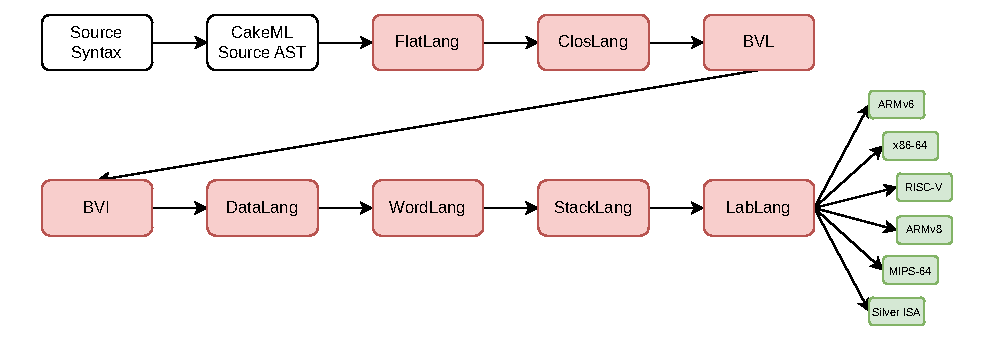
\includegraphics[width=\linewidth]{images/cake.pdf}
    \caption{\cml multi-stage pipeline}
    \label{fig:CakeMLPipeline}
\end{figure}

In the figure \ref{fig:CakeMLPipeline} the red boxes represent all the languages the compiler passes through until it reaches the
encoding for each of the different types of machine code programs, represented as green.

\subsection{PureCake}

Another tool that compiles to \cml code with a verified compiler is PureCake, which is a HOL4-verified compiler for a lazy, 
functional language with Haskell-like, indentation sensitive syntax. Since, the output code is \cml code it can be passed 
through \cml trusted backend, ensuring end-to-end verification~\cite{KanabarVAMNPZ23}.

Inspired by \compcert, it targets a Standard ML-style language and compiles down to \cml through a verified pipeline.
This design not only makes it possible to compile lazy functional programs in a sound and verified way, but also showcases 
how flexible \cml's verified infrastructure can be when adapting to different programming language styles. 
By supporting features that are rarely seen in other verified compilers, PureCake expands the range of languages that can 
benefit from verified compilation, showing that it's feasible to bring formal guarantees even to non-strict, high-level 
functional languages~\cite{KanabarVAMNPZ23, KanabarKM24}.

\section{Pipeline}
\label{sec:Pipeline}

In this section we reintroduce the \cameleer pipeline found in figure \ref{fig:CameleerPipeline}, but now with some slight changes
to accommodate the extraction mechanism from \whythree :

\begin{figure}[H]
    \centering
    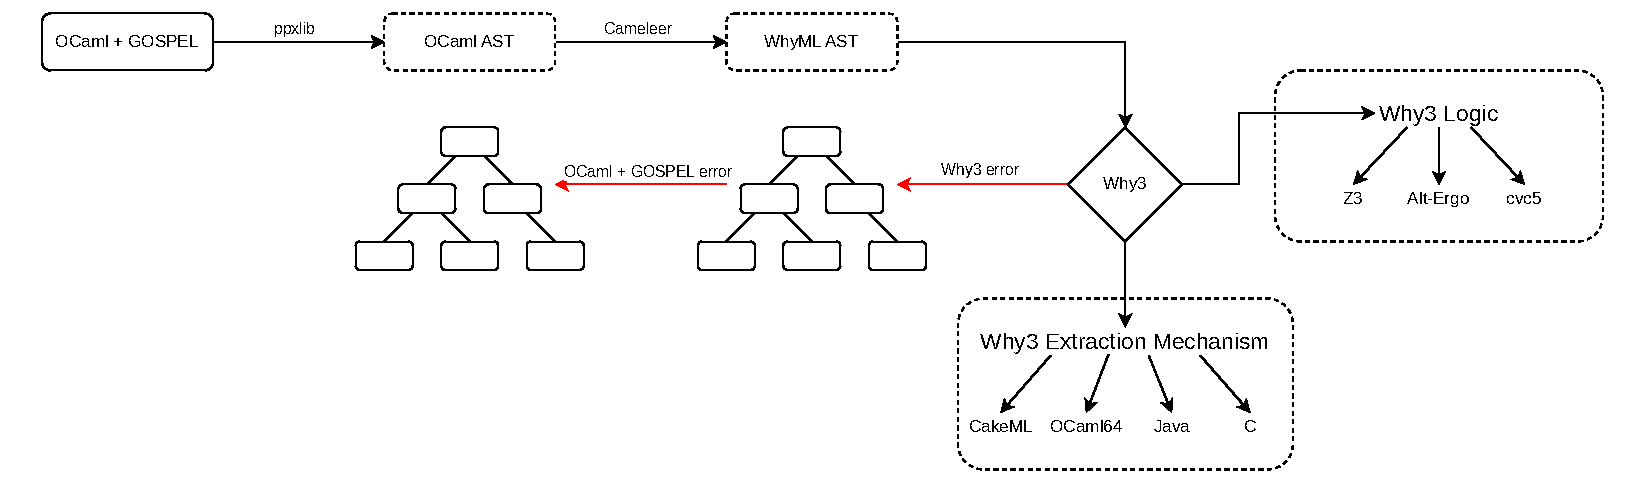
\includegraphics[width=\linewidth]{images/cameleer_extract.pdf}
    \caption{\ocaml to \whyml pipeline with \cameleer}
    \label{fig:Cameleer_pipeline}
\end{figure}

A brief explanation for the extended \cameleer pipeline, is that \cameleer translates \ocaml programs with \gospel annotations to 
\whyml language internally, on one hand if an error is caught relating to \ocaml or \whyml it will be handled accordingly, on the 
other hand if there is no syntax error the \whythree platform is initialized and the provers can be used to verify the proof goals.

The extraction mechanism introduced in the figure \ref{fig:Cameleer_pipeline} is separate from the verification process.
This means that a program may be extracted to another language without requiring the correctness of the code to be proven, 
the only guarantee is that the program does have any \ocaml or \gospel compilation errors. 
This may lead to extraction of potentially incorrect \ocaml programs, with the full responsibility of extracting after proving the
code falling on the user's side. 

The initial objective of the extraction mechanism was to build correct by construction libraries with the help of \whythree. This lead
to the creation of a mechanism that in itself does not jeopardize the behaviour of the original code when translating, this is due to its 
mathematical formalization~\cite{Pereira18}. One of the main advantages is the existence of a dedicated phase for the removal of ghost code and logical
annotations present in the original \whyml code, in addition to a few conservative optimizations. The resulting code does not contain 
any logical elements which facilitates the translation to a new language, this means the only effort that needs to be done
is similar to writing a printer from an intermediate representation of the language to be added~\cite{Pereira18}. Currently, four languages 
are allowed to be extracted from \whyml while using the \whythree platform, these are C, Java, \ocaml (OCaml64) and 
\cml~\cite{Why3Extract, Pereira18}.